\documentclass{beamer}
\usepackage{slides}

\newcommand{\pic}[3][0.5]{
\begin{frame}
    #2
    \begin{figure}
        \centering
        \includegraphics[width=#1\linewidth]{#3}
    \end{figure}
\end{frame}
}

\title{Avoiding sillies}

\begin{document}

\frame{\titlepage}

\begin{frame}
    \frametitle{A motivating quote}
    \begin{quote}
        \sffamily\small
        To succeed in competition math it is not enough to be right. It is also necessary to not be wrong.
    \end{quote}
\end{frame}

\begin{frame}
    \frametitle{What is a silly?}
    \begin{definition}
        A \emph{silly} is an almost-correct solution with a ``dumb'' mistake.
    \end{definition}
    Sillies are Minnetonka's downfall.
\end{frame}

\begin{frame}
    \frametitle{Examples}
    \begin{definition}
        A \emph{silly} is an almost-correct solution with a ``dumb'' mistake.
    \end{definition}
    \begin{itemize}
        \ii Arithmetic mistakes
        \ii Forgetting edge cases
        \ii Misreading the question
        \ii Sign errors
        \pit Listening to a song with a number and writing that instead
    \end{itemize}
\end{frame}

\begin{frame}
    \frametitle{Non-examples}
    \begin{definition}
        A \emph{silly} is an almost-correct solution with a ``dumb'' mistake.
    \end{definition}
    Significant mistakes are not sillies. If there are $n$ problems and you scored $m$, you didn't silly $n - m$ problems.
    \begin{itemize}
        \ii Fundamentally flawed approach
        \ii Failed guess
        \pit Answer sheet spontaneously catches fire
        \pit Accidentally eat chocolate containing alcohol before the contest
    \end{itemize}
\end{frame}

\begin{frame}
    \frametitle{The problem}
    Sillies are easily correctable.

    \begin{corollary}
        Reducing sillies is an easy way to improve.
    \end{corollary}

    Example: Me at HMMT 2025
    % HMMT 2025 story: 60 percent increase in total indivs solved without sillies (646 -> 226)
\end{frame}

\begin{frame}
    \frametitle{Factors increasing sillies}
    \begin{itemize}
        \ii Doing problems quickly (Me at ARML tiebreaks 2025)
        % Three tiebreaker problems, I sillied p1 and p2 by making two consecutive sign errors.
        % I proceeded to misread the third one. This cost me a lot of money.
        % I needed the money to buy dinner since I gambled away my alloted dinner money the previous night.
        % It's okay though, since I sold my medal to Mark Shi for 50 dollars.
        \ii Headsolving or solving with low scratch paper
        \ii Sleep deprivation or jet lag
        \ii Strong, distracting emotions, such as excitement, anger, or heartbreak
        \ii Sickness
        \pit Doing problems under the influence (don't drink and derive)
        \pit Having family history of sillying
    \end{itemize}
\end{frame}

\begin{frame}
    \frametitle{Factors \st{increasing} \alert{decreasing} sillies} % TODO: fix
    \begin{itemize}
        \ii Doing problems \st{quickly} \alert{slowly}
        \ii \st{Headsolving or solving with low scratch paper} \alert{using scratch paper liberally}
        \ii \st{Strong, distracting emotions, such as excitement, anger, or heartbreak} \alert{being locked in}
    \end{itemize}
\end{frame}

\begin{frame}
    \frametitle{Most important advice}
    \alert{Reasoning must be PAINFULLY explicit.} Smart people make stupid mistakes. Write down all reasoning. Do not skip steps in your head!

    \medskip

    Slow is smooth, smooth is fast. Sillies when barying ISL 2024 G4 turned $20$ minutes into $3$ hours.
\end{frame}

\begin{frame}
    \frametitle{Pointing-and-calling}
    \begin{itemize}
        \ii In many Asian railways, conductors are required to literally point and call out what they're seeing and doing
        \ii Sounds dumb? Shown to reduce error by $85\%$
        \ii Being painfully explicit reduces errors
    \end{itemize}
\end{frame}

\begin{frame}
    \frametitle{The pointing-and-calling method}
    \begin{figure}
        \centering
        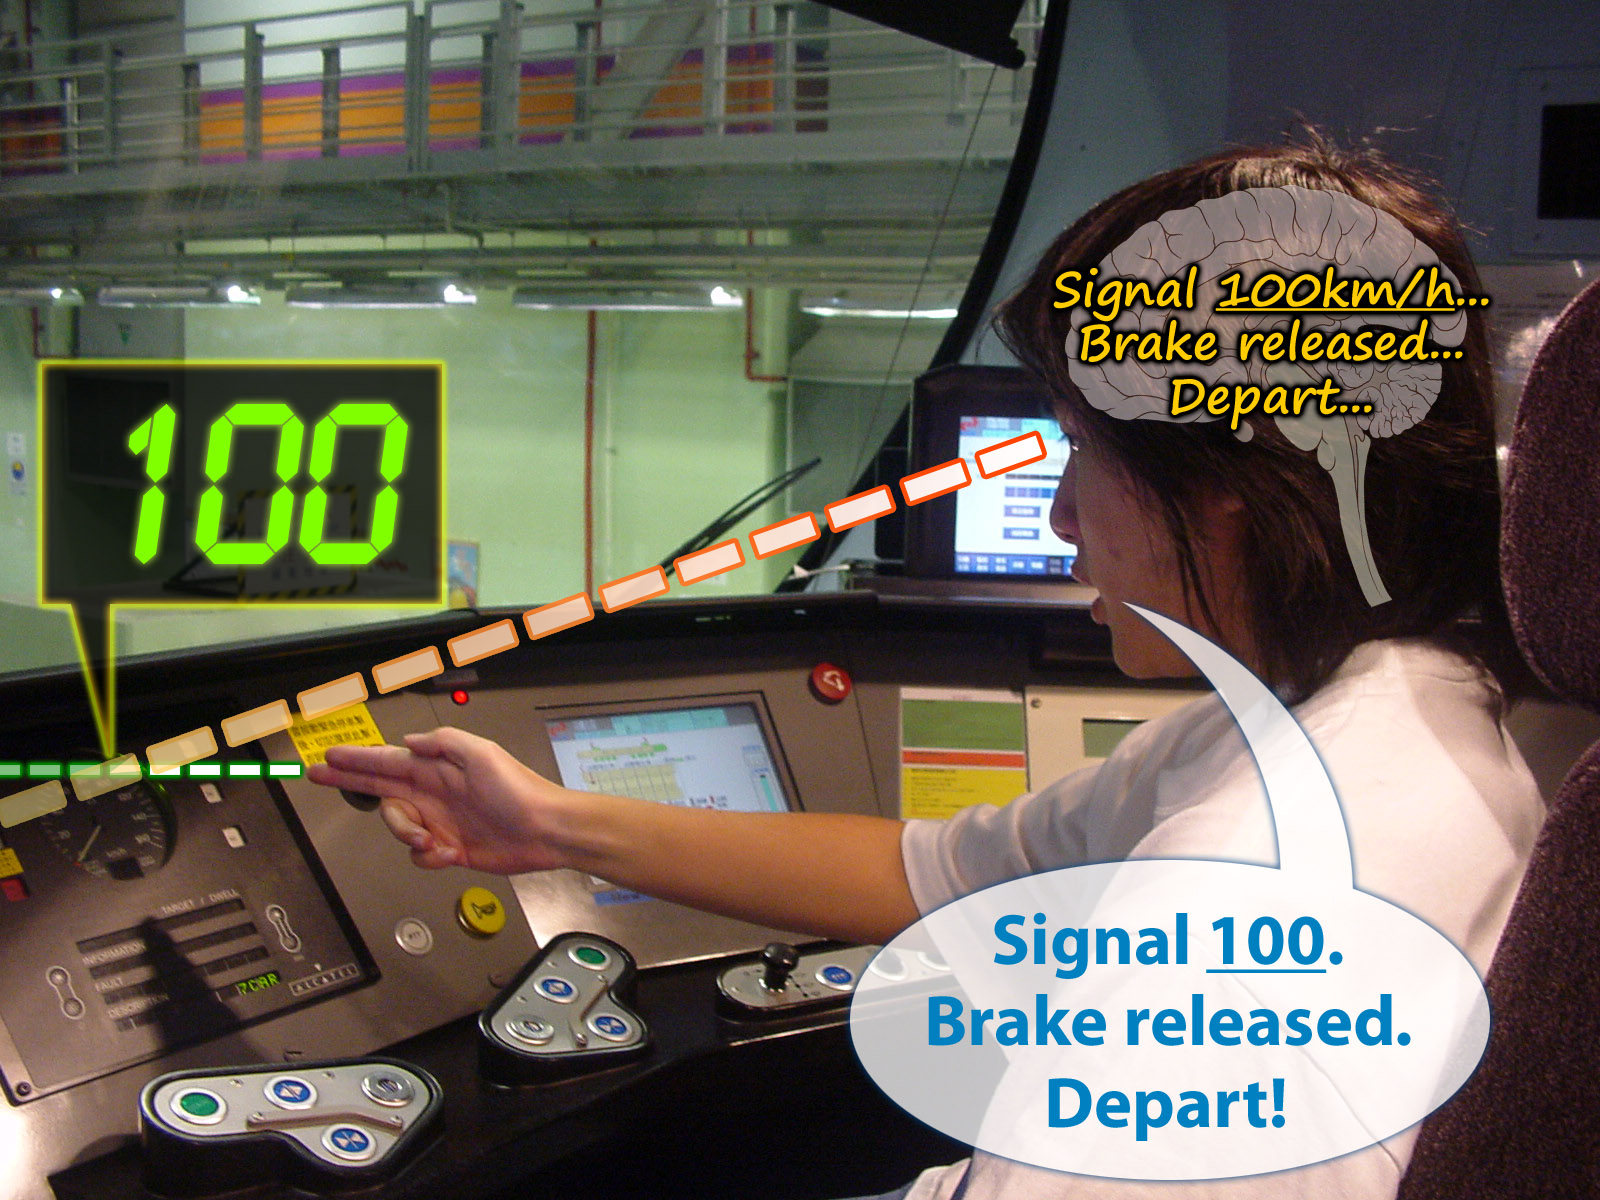
\includegraphics[width=0.7\linewidth]{pointing-and-calling.jpg}
        \caption{The process of pointing and calling. Image from Wikipedia.}
    \end{figure}
\end{frame}

\begin{frame}
    \frametitle{Good and bad scratchwork}
    Scratchwork isn't only for computation. Work out small examples. Write down reasoning.

    \medskip

    Writing \alert{everything} down is pointing-and-calling. If you think $2 \times 3$, don't write $6$. Don't skip steps!

    \medskip

    Don't use test paper margins (not enough space). You'll write over yourself and problems. You are not Fermat.
\end{frame}

\begin{frame}
    \frametitle{Good and bad scratchwork}
    The following slides include examples of scratch paper.

    \medskip

    Think about how their paper is organized and how work is being done.
\end{frame}

\pic{Lanie Deng}{lanie-scratch.jpg}
\pic[0.9]{Michael Luo}{michael-scratch1.jpg}
\pic[0.9]{Michael Luo}{michael-scratch2.jpg}
\pic[0.9]{Michael Luo}{michael-scratch3.jpg}
\pic[0.9]{Michael Luo}{michael-scratch4.jpg}
\pic[0.9]{Michael Luo}{michael-scratch5.jpg}
\pic[0.9]{Michael Luo}{michael-scratch6.jpg}
\pic{Selena Ge}{selena-scratch.jpg}
\pic[0.6]{Evan Chen}{greta-scratch.jpg}
\pic{Jiahe Liu}{john-scratch.jpg}
\pic{Catherine Xu}{catherine-scratch.jpg}
\pic{Andrew Lin}{andrew-scratch.jpg}
\pic{\href{https://open.spotify.com/track/0fKkmR53Rn3T9iUwb2iG20?si=194f7109176e43b2}{Alexander Wang}}{alex-scratch.jpg}

\begin{frame}
    \frametitle{Practice meet today}
    We'll do Sample Meet 4 Coyote. Write down reasoning in words. I'll check! If you do not do this, you will face execution.

    \medskip

    Good luck!
\end{frame}

\end{document}